%%
% Please see https://bitbucket.org/rivanvx/beamer/wiki/Home for obtaining beamer.
%%
\documentclass[aspectratio=169]{beamer}
\usetheme{Antibes}
\usepackage{xcolor}
\mode<presentation>

\useoutertheme{miniframes} 
\useinnertheme{circles}

\definecolor{primary}{HTML}{003469}
\definecolor{secondary}{HTML}{003469}
\definecolor{tertiary}{HTML}{00addc}

\setbeamercolor{titlelike}{bg=white,fg=primary}

\setbeamercolor{palette primary}{bg=tertiary,fg=white}
\setbeamercolor{palette secondary}{bg=tertiary,fg=white}
\setbeamercolor{palette tertiary}{bg=secondary,fg=white}
\setbeamercolor{structure}{fg=secondary} % itemize, enumerate, etc
\setbeamercolor{section in toc}{fg=secondary} % TOC sections
% Override palette coloring with secondary
\setbeamercolor{subsection in head/foot}{bg=tertiary,fg=white}
\usepackage{natbib}
\bibliographystyle{unsrtnat}
\setcitestyle{authoryear,open={(},close={)}}
\usepackage{csquotes}


\title{\large{\textbf{Python, Cloud and Automation}} \newline\newline 1. Introduction}

\author{Jack Minchin}
\institute{Tourism Economics}
\date{2022}

\begin{document}

\frame{\titlepage}

\begin{frame}
\frametitle{Table of Contents}
\tableofcontents
\end{frame}

\section{Introduction}

\begin{frame}{Outline}
	\begin{enumerate}
		\item \textbf{3rd March - Morning}
		\begin{itemize}
		\item Part 1: Introduction
			\begin{itemize}
			\item What is Python?
			\item How can it be used?
			\item How can I learn?
		\end{itemize}
		
		\item Part 2: Getting Started
		
		\begin{itemize}
  			\item Downloading
  			\item Writing
  			\item Managing Projects
  			\item Some basic examples
		\end{itemize}
		
		
		\end{itemize}
		
		\item \textbf{3rd March - Afternoon}
		
		\begin{itemize}
  		 	\item Part 3: Automation, Cloud and Examples
  		 	\begin{itemize}
			  \item What are cloud technologies and how are they used?
			  \item What are pipelines?
			  \item 3 Examples of automation
		\end{itemize}
		\end{itemize}

	

	\end{enumerate}
\end{frame}


\begin{frame}{What Python is not}
\framesubtitle{Some common misconceptions}

\begin{itemize}
	\item A statistical package
	\item A program
	\item A self contained framework
\end{itemize}

\end{frame}


\begin{frame}{What is Python?}
\blockquote[wikipedia]{
	Python is a high-level, general-purpose programming language. Its design philosophy emphasizes code readability with the use of significant indentation. Its language constructs and object-oriented approach aim to help programmers write clear, logical code for small- and large-scale projects.}
\end{frame}

\section{Some Use-Cases}

\begin{frame}{How can we use it?}

\begin{enumerate}
	\item \textbf{Extraction, Transform and Load (ETL) Tasks}

			Reading data from (virtually) any source, transforming into required format and exporting.
	
	\item \textbf{Automation of repetitive tasks.}
	
			Interacting with file system, using libraries to create PowerPoints, interacting directly with excel, read emails - the possibilities really are endless.
			
	\item \textbf{Data Visualisation, Analysis and Econometrics}
	
	\item \textbf{Full scale applications}
		
			Larger projects will span multiple categories (e.g Country Profile Report automation)\footnote{Current implementation uses another language called JavaScript (Node.js) for the PDF generation.}
	
\end{enumerate}
	
\end{frame}

\begin{frame}{Where can we use Python, Automation \& Cloud}

\begin{itemize}
\item Automating and creating outputs in PDF, Excel and PowerPoint formats.

 		{\small e.g Whitbread Quarterly, Jessie's regular outputs, Sweden Regional TSA, GTS Country Profiles, GCT City Reports}
 		
\item Python as a `glue code'

	{\small e.g small scripts to glue wider projects / models together.}
 		
 \item {Automating regular data inputs and reading on to the model.} 
 
 		{\small e.g IATA data processing, STR Data ingestion etc.}
 		
 \item{Automating test and checks on model outputs}
 
	 {\small e.g APF and GTS output checks (no negatives etc.)}
	 
	 
 \item{Storing data in the cloud}
 
	 {\small e.g Latest model always uploaded to cloud storage to allow cloud extracts in pipelines, all data extract stored in database to allow quick pulls in model workbooks.}
 		
\end{itemize}
\end{frame}

\begin{frame}{Where can we use it}

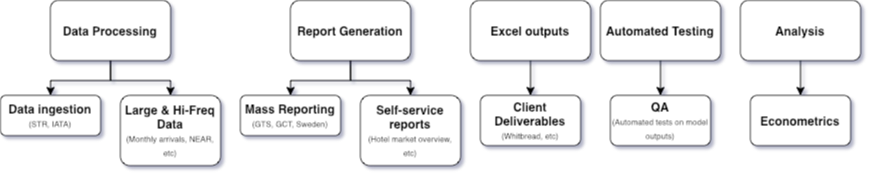
\includegraphics[width=\linewidth]{graphics/projects.drawio.png}
	
\end{frame}


\begin{frame}{A general note}

{\Large While Python is great for some use cases, particularly \textbf{data processing} and \textbf{analysis}, the main objective over the next few days is to bring about more awareness for automation in general, which is language agnostic - but Python is a good place to start.}
	
\end{frame}



\section{Resources for learning}

\begin{frame}{How to learn Python}

\begin{enumerate}

\item \textbf{Learning-by-doing}

		The \textbf{best} way to learn Python is to start writing it. There are multiple courses online, from free YouTube videos to paid courses but in-person courses will not help unless you are spending hours working alone figuring out.
		
\item \textbf{DataCamp.com}
	
		Combines very short videos with active excercices, it teaches concepts in a concise way and then forces you to get involved. It is also designed for ETL, statistics and data science. 

	
\end{enumerate}
\end{frame}





\end{document}
